\documentclass[journal]{IEEEtran}
\usepackage{graphicx}  % Written by David Carlisle and Sebastian Rahtz
\usepackage{amsmath}
\usepackage{color}
\usepackage{hyperref}
\hyphenation{op-tical net-works semi-conduc-tor IEEEtran}
\def\le{\left}
\def\ri{\right}
\def\nnnl{\nonumber\\}
\def\um{\,\mu\mathrm{m}}
\def\comment#1{{\sf #1\/}} 
% paper title
\begin{document}
\title{A Simulation Circuit to Characterize Transistors}
\author{Christoph Maier~\IEEEmembership{Member,~IEEE}% <-this % stops a space
\thanks{Copyright \copyright\ 2008, 2014, 2019 under Creative Commons
Attribution-NonCommercial-ShareAlike 4.0 International (CC BY-NC-SA 4.0) license.}}%
%~\ref{http://creativecommons.org/licenses/by-nc-sa/4.0/}}% <-this % stops a space
\maketitle
\begin{abstract}\boldmath
I present a simple simulation schematic to extract transistor parameters relevant for analog circuit design:
transconductance~$g_m$, transconductance per current~$g_m/I_d$, and voltage gain~$g_m/g_o$.
\end{abstract}


\begin{IEEEkeywords}
SPICE, LTspice, MOSFET, process characterization, $g_m/I_d$ design method
\end{IEEEkeywords}

\IEEEpeerreviewmaketitle
%%
\section{The circuit}
%%
\begin{figure}[h]
\centering
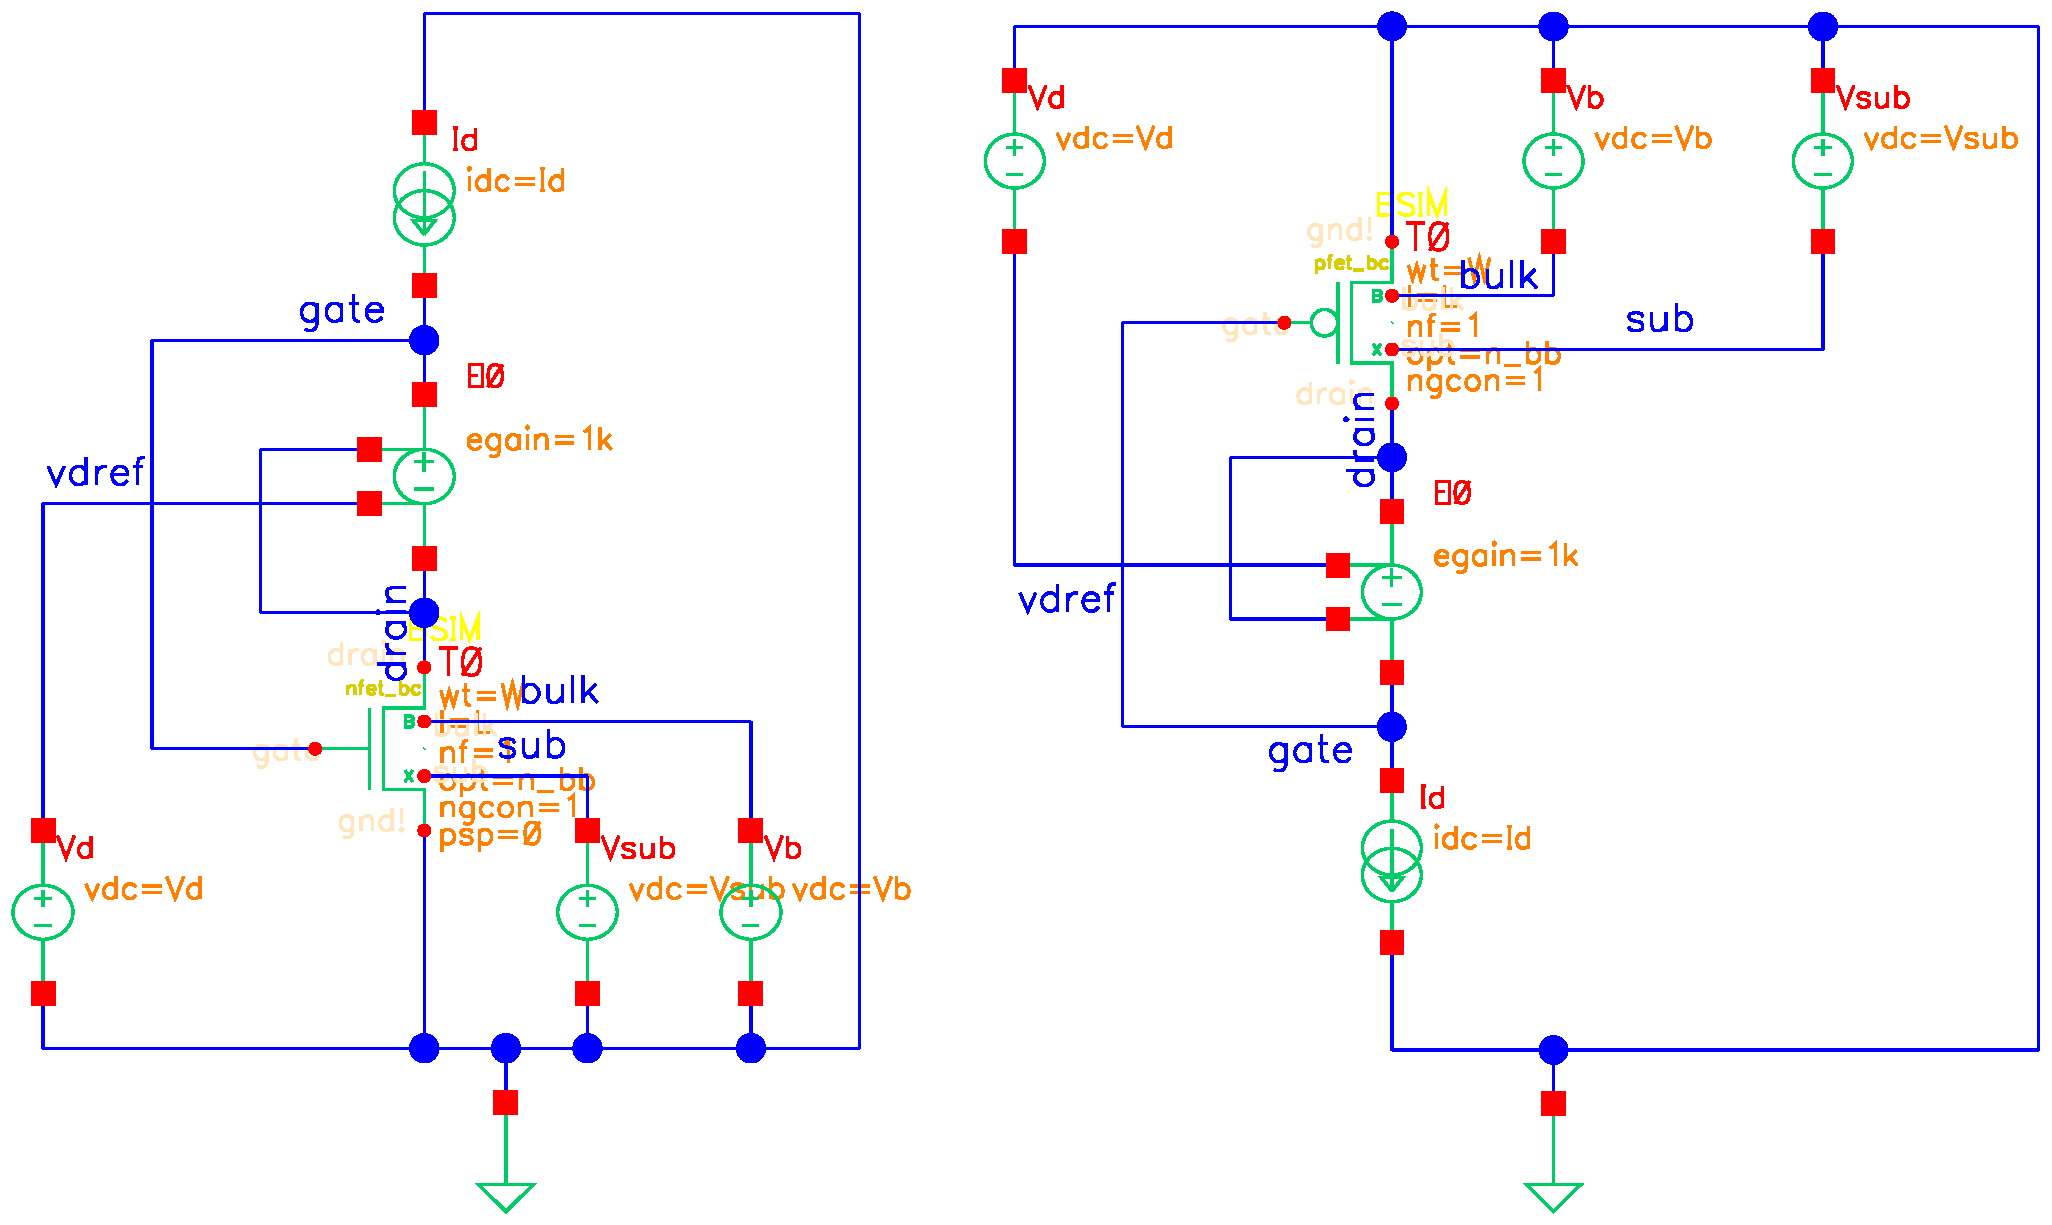
\includegraphics[width=1.0\columnwidth]{figures/mostest_fb.pdf}
\caption{Simulation schematics to characterize MOSFETs}
\label{fig:schematics}
\end{figure}
%
The main design parameters for dimensioning MOSFETs are their drain current~$I_d$, 
which controls transconductance, 
and the drain-to-source voltage~$V_{ds}$, which controls output conductance~$g_o$.
However, the operating point of the transistor is controlled mostly by the gate-to-source voltage~$V_{gs}$, which varies a lot between different wafers of the same IC design.

I solve this by regulating the gate voltage by a feedback loop
that adjusts $V_g$ to set the drain voltage $V_d$ to a reference $V_{d,ref}$ 
by an ideal voltage controlled voltage source (VCVS) with voltage gain~$A$. 
The schematics for the NMOS and PMOS simulation circuits are shown in Figure~\ref{fig:schematics}. 

Kirchhoff's Current Law yields the small-signal equations
\begin{IEEEeqnarray}{c}
I_d = g_m V_g + g_o V_d \label{eqn:KCL}\\
V_g = V_d + A \le(V_d - V_{d,ref}\ri) \nonumber
\end{IEEEeqnarray}
which lead to
\begin{equation}\label{eqn:Vg}
V_g = \frac{I_d-g_o\,V_{d,ref}\,A/\le(1+A\ri)}{g_m + g_o/\le(1+A\ri)}
\end{equation} 
and
\begin{equation}\label{eqn:Vd}
V_d = \frac{I_d+A\,g_m\,V_{d,ref}}{\le(1+A\ri) g_m + g_o}\,.
\end{equation} 

In the ideal case of $A\rightarrow\infty$, 
\begin{equation}\label{eqn:Vg_ideal}
V_g = \frac{I_d-g_o\,V_{d,ref}}{g_m}
\end{equation} 
and
\begin{equation}\label{eqn:Vd_ideal}
V_d = V_{d,ref}\,.
\end{equation} 

\section{Parameter extraction}
%%
\subsection{Transconductance}
%
The transconductance $g_m$ as function of drain current can be obtained 
by sweeping $I_d$ for fixed $V_d$, as 
\begin{equation}\label{eqn:gm}
1/\le(\frac{\partial V_g}{\partial I_d}\ri) = g_m+g_o/\le(1+A\ri) 
\overset{A\rightarrow\infty}{\approx} g_m\,.
\end{equation}

\subsection{$g_m/I_d$}
%
The specific transconductance $g_m/I_d$ is a useful design parameter 
for setting the bias point of a transistor~\cite{Silveira1996}. 
$g_m/I_d$ is maximal in subthreshold operation. 
It is obtained by sweeping $I_d$ for fixed $V_d$ and calculating
\begin{equation}\label{eqn:gm_over_Id}
1/\le(\frac{\partial V_g}{\partial I_d}\,I_d\ri) = \frac{g_m+g_o/\le(1+A\ri)}{I_d}
\overset{A\rightarrow\infty}{\approx} \frac{g_m}{I_d}\,.
\end{equation}

\subsection{$g_m/g_o$}
%
While $g_m$ or $g_m/I_d$ is the most important design criterion for dimensioning a transistor,
the next most important criterion is setting the output conductance $g_o$. 
With the circuits in Figure~\ref{fig:schematics}, 
the intrinsic voltage gain $g_m/g_o$ can be extracted by sweeping $V_{d,ref}$ for constant $I_d$.
\begin{equation}\label{egn:gm_over_go}
-\le(\frac{\partial V_d}{\partial V_{d,ref}}\ri)
/\le(\frac{\partial V_g}{\partial V_{d,ref}}\ri)
= \frac{\frac{A\,g_m}{\le(1+A\ri)g_m+g_o}}{\frac{A\,g_o}{\le(1+A\ri)g_m+g_o}} 
= \frac{g_m}{g_o} \,.
\end{equation}

\section{Parameter sweeps}
%%
\subsection{Transconductance}
%
Even when MOS transistor models are too complicated for hand calculations,
the specific transconductance $g_m/I_d$ indicates
the operating region of the transistor~\cite{Silveira1996}.
 
In the weak inversion region, $I_d$ is an exponential function of $V_g$,
\begin{equation}
I_d = I_{d{0}} \exp\le(\frac{q}{n\;k\,T}\le(V_g-V_t\ri)\ri)
\end{equation}
with $V_t$~the threshold voltage, $q$~the electron charge, $k$~the Boltzmann constant, 
$T$~the absolute temperature, $n>1$~a process dependent factor, 
and $I_{d{0}}$~a proportionality constant depending on geometry,
so
\begin{equation}
\frac{g_m}{I_d}
= \frac{\frac{\partial I_d}{\partial V_g}}{I_d} 
= \frac{\frac{q}{n\;k\,T} I_{d{0}} \exp\le(\frac{q}{n\;k\,T}\le(V_g-V_t\ri)\ri)}
       {I_{d{0}} \exp\le(\frac{q}{n\;k\,T}\le(V_g-V_t\ri)\ri)}
= \frac{q}{n\;k\,T}\,.
\end{equation}

In the strong inversion region, $I_d$~depends quadratically on~$V_g$,
\begin{equation}
I_d = \frac{\kappa}{2}\le(V_g-V_t\ri)^2
\end{equation}
with the threshold voltage~$V_t$ and a geometry and process dependent factor~$\kappa$,
so 
\begin{equation}
\frac{g_m}{I_d}
= \frac{\kappa\le(V_g-V_t\ri)}{\frac{\kappa}{2}\le(V_g-V_t\ri)^2}
= \frac{2}{V_g-V_t}
\end{equation}
where $V_g-V_t > 2\,\frac{n\;k\,T}{q}$ for the transistor to be above weak inversion.

With a logarithmic dc sweep of~$I_d$ at a given~$V_d$, the transition between weak and strong inversion can be seen by $g_m/I_d$ falling from its essentially constant value for weak inversion at the onset of strong inversion. 
$g_m$ is obtained by taking the derivative with respect to the dc sweep variable $I_d$ 
of both $V_g$ and~$I_d$.
This is shown in LT\,Spice\,IV for two different processes 
(TSMC~250\,nm and TSMC~180\,nm) in Figures \ref{fig:gm_mos25} and~\ref{fig:gm_mos18}. 

%
\begin{figure}[h]
\centering
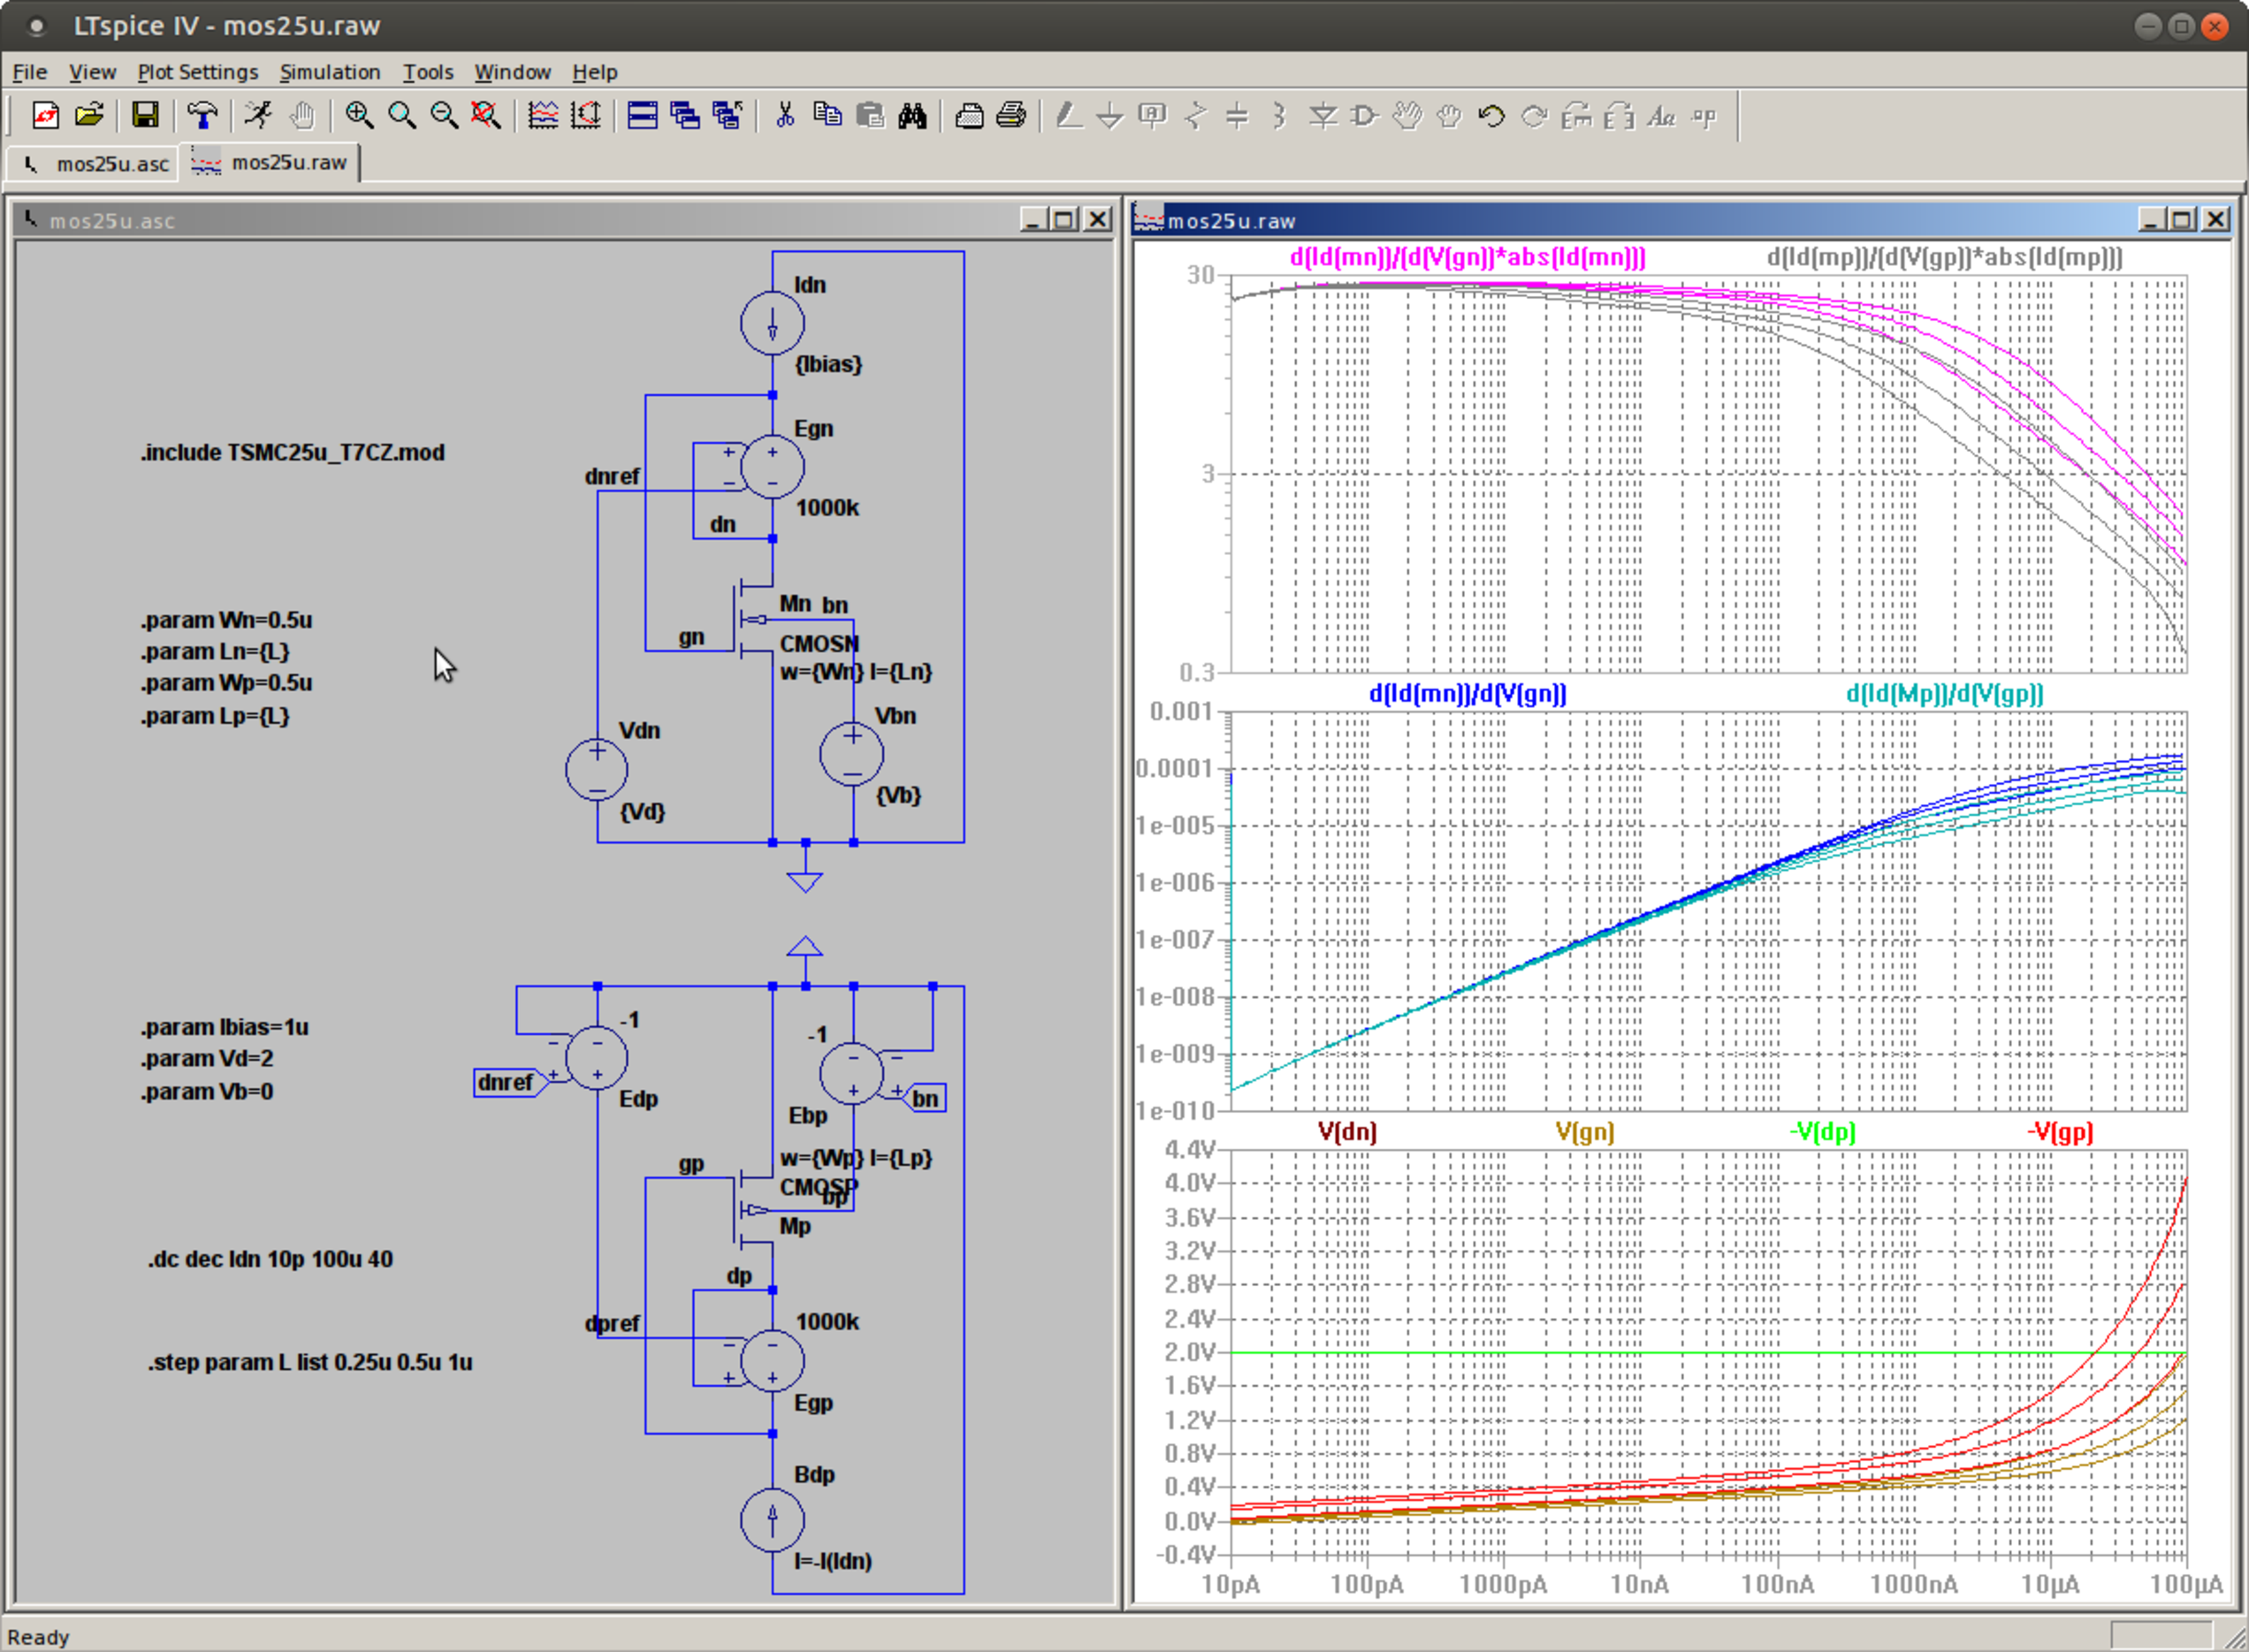
\includegraphics[width=1.0\columnwidth]{figures/mos25u.pdf}
\caption{Transconductance characterization for 250\,nm process}
\label{fig:gm_mos25}
\end{figure}
%
\begin{figure}[h]
\centering
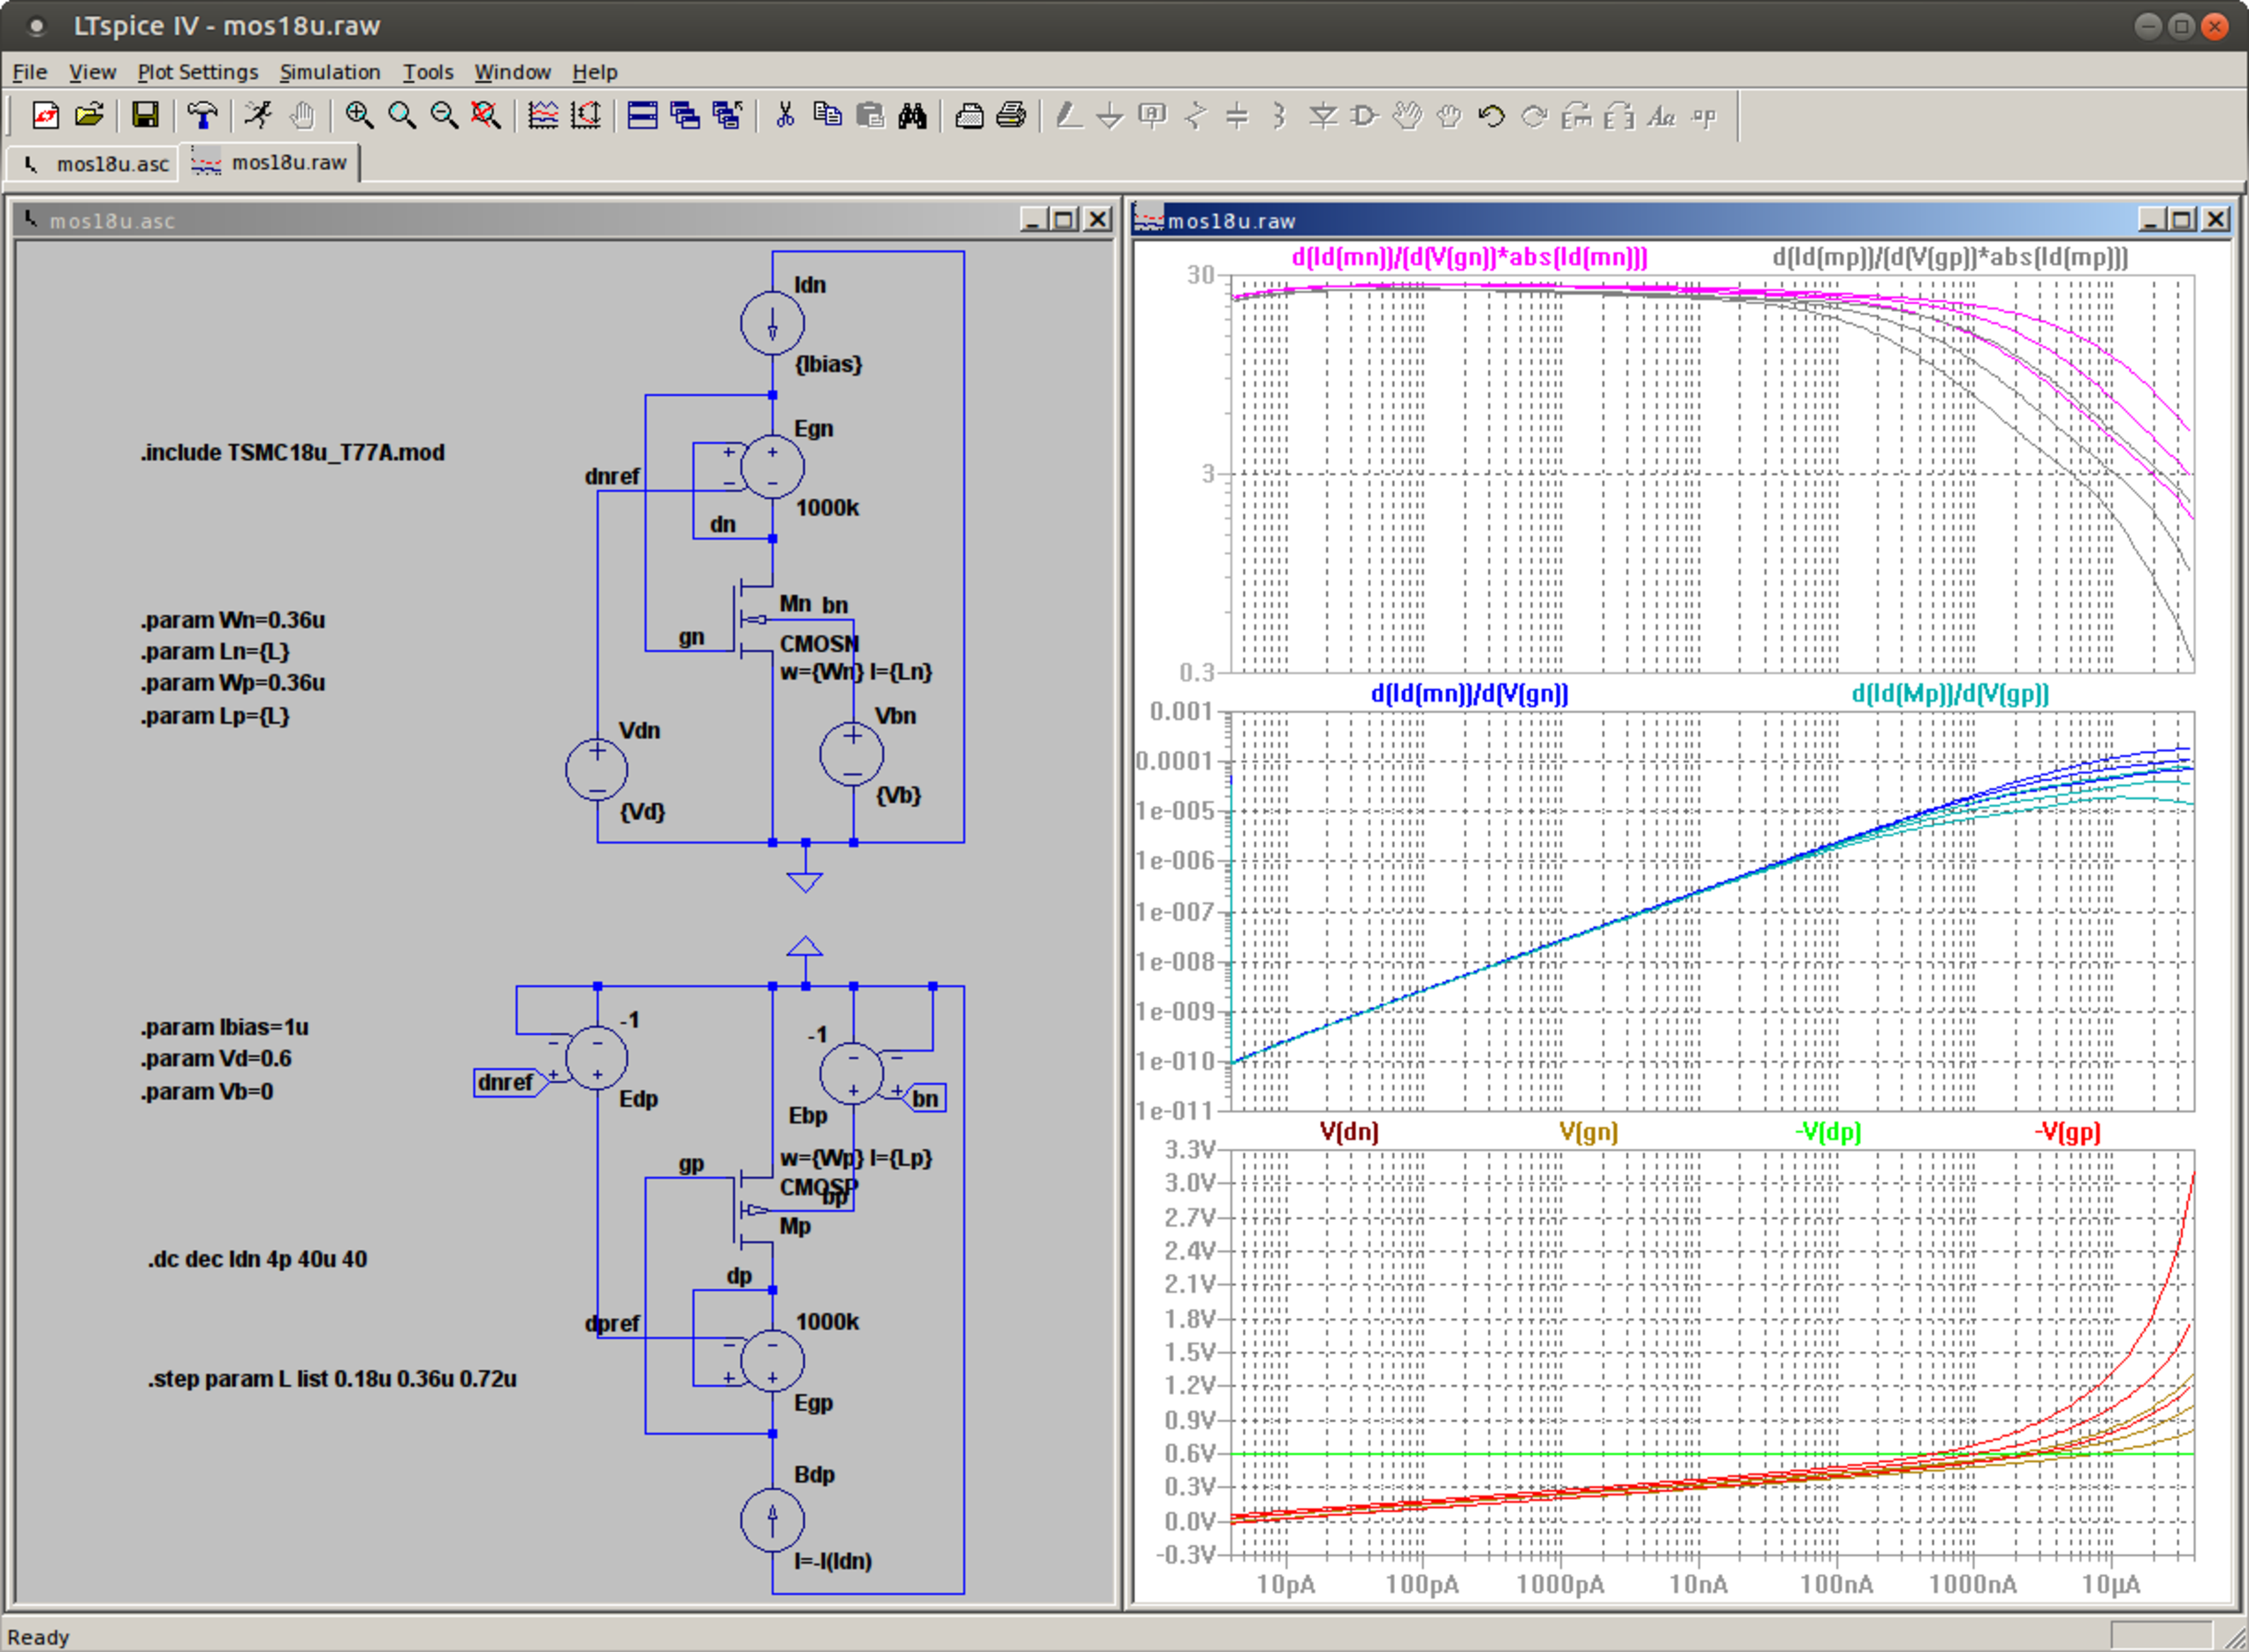
\includegraphics[width=1.0\columnwidth]{figures/mos18u.pdf}
\caption{Transconductance characterization for 180\,nm process}
\label{fig:gm_mos18}
\end{figure}
%

For smaller $W/L$ ratios, $g_m/I_d$ starts dropping at lower $I_d$, 
and for the same $W/L$ ratio, the $g_m/I_d$ of PMOS transistors starts dropping at lower $I_d$ than NMOS due to the lower mobility of holes vs.\ electrons.

For low-power, low noise circuits, 
the signal amplifying transistors should be dimensioned and biased in weak inversion
near the onset of moderate inversion. 

\subsection{Voltage gain}
%
\begin{figure}[h]
\centering
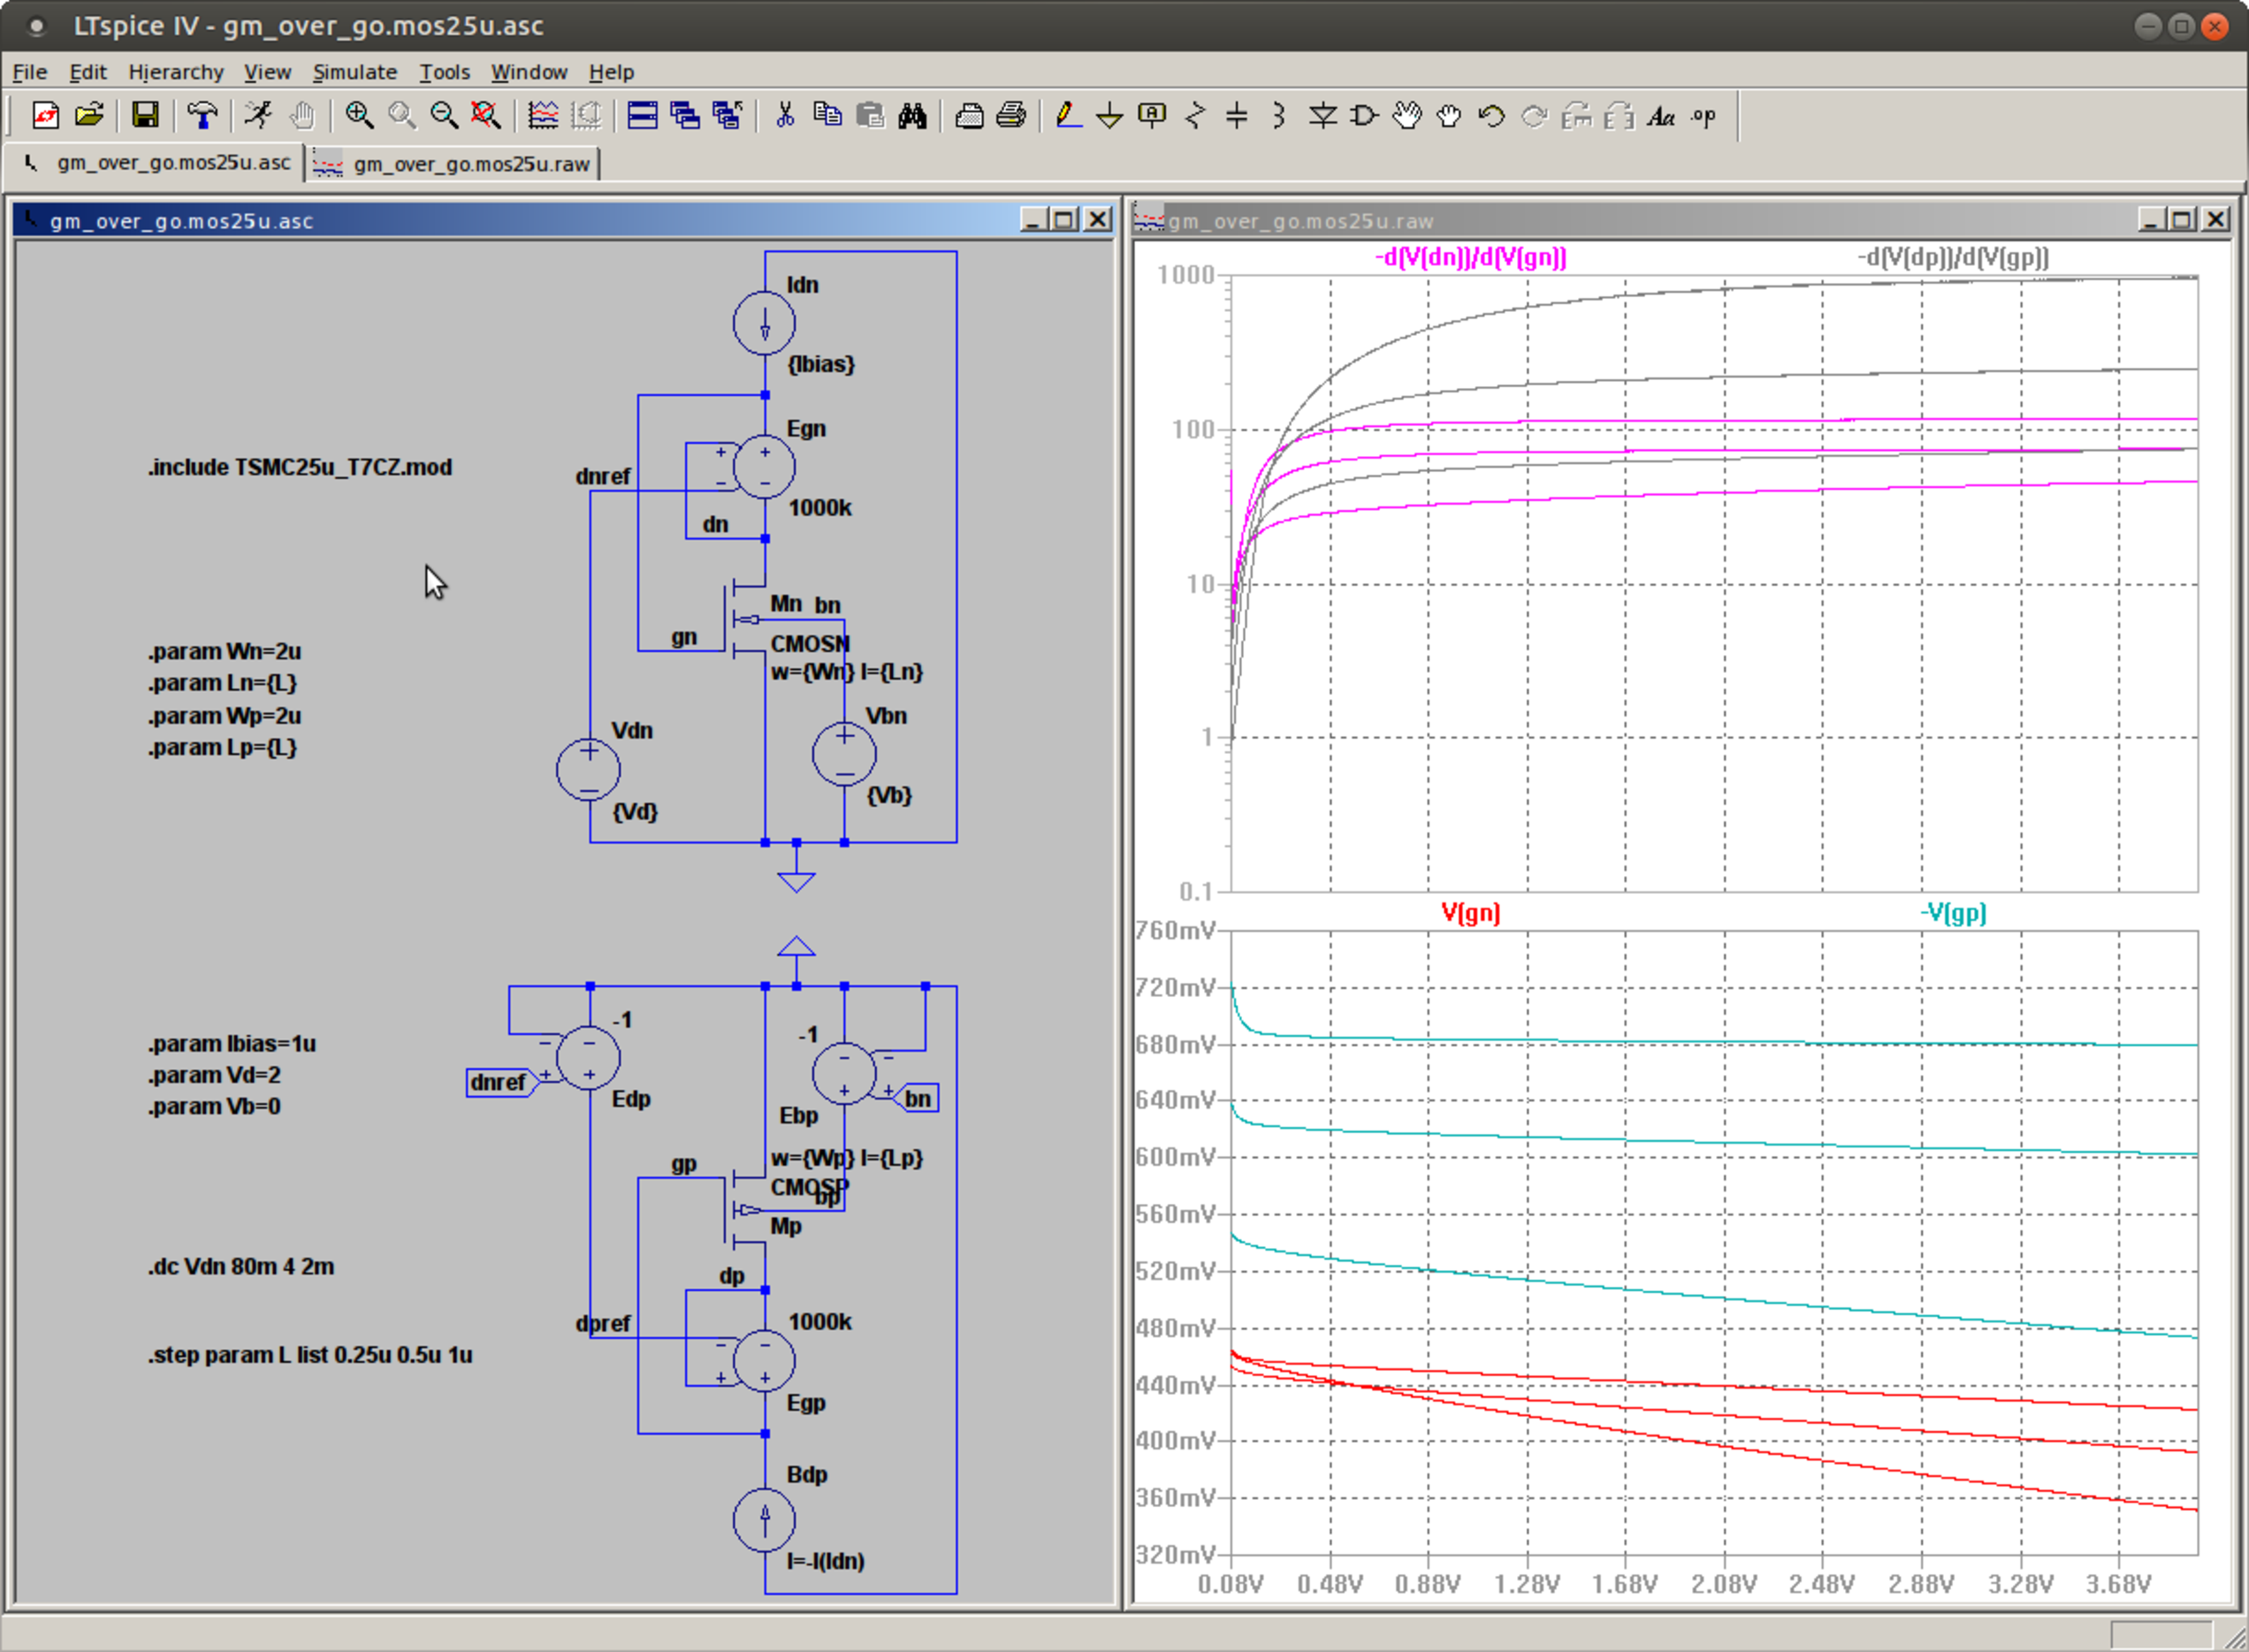
\includegraphics[width=1.0\columnwidth]{figures/gm_over_go_mos25u.pdf}
\caption{Voltage gain characterization for 250\,nm process}
\label{fig:gm_go_mos25}
\end{figure}
%
\begin{figure}[h]
\centering
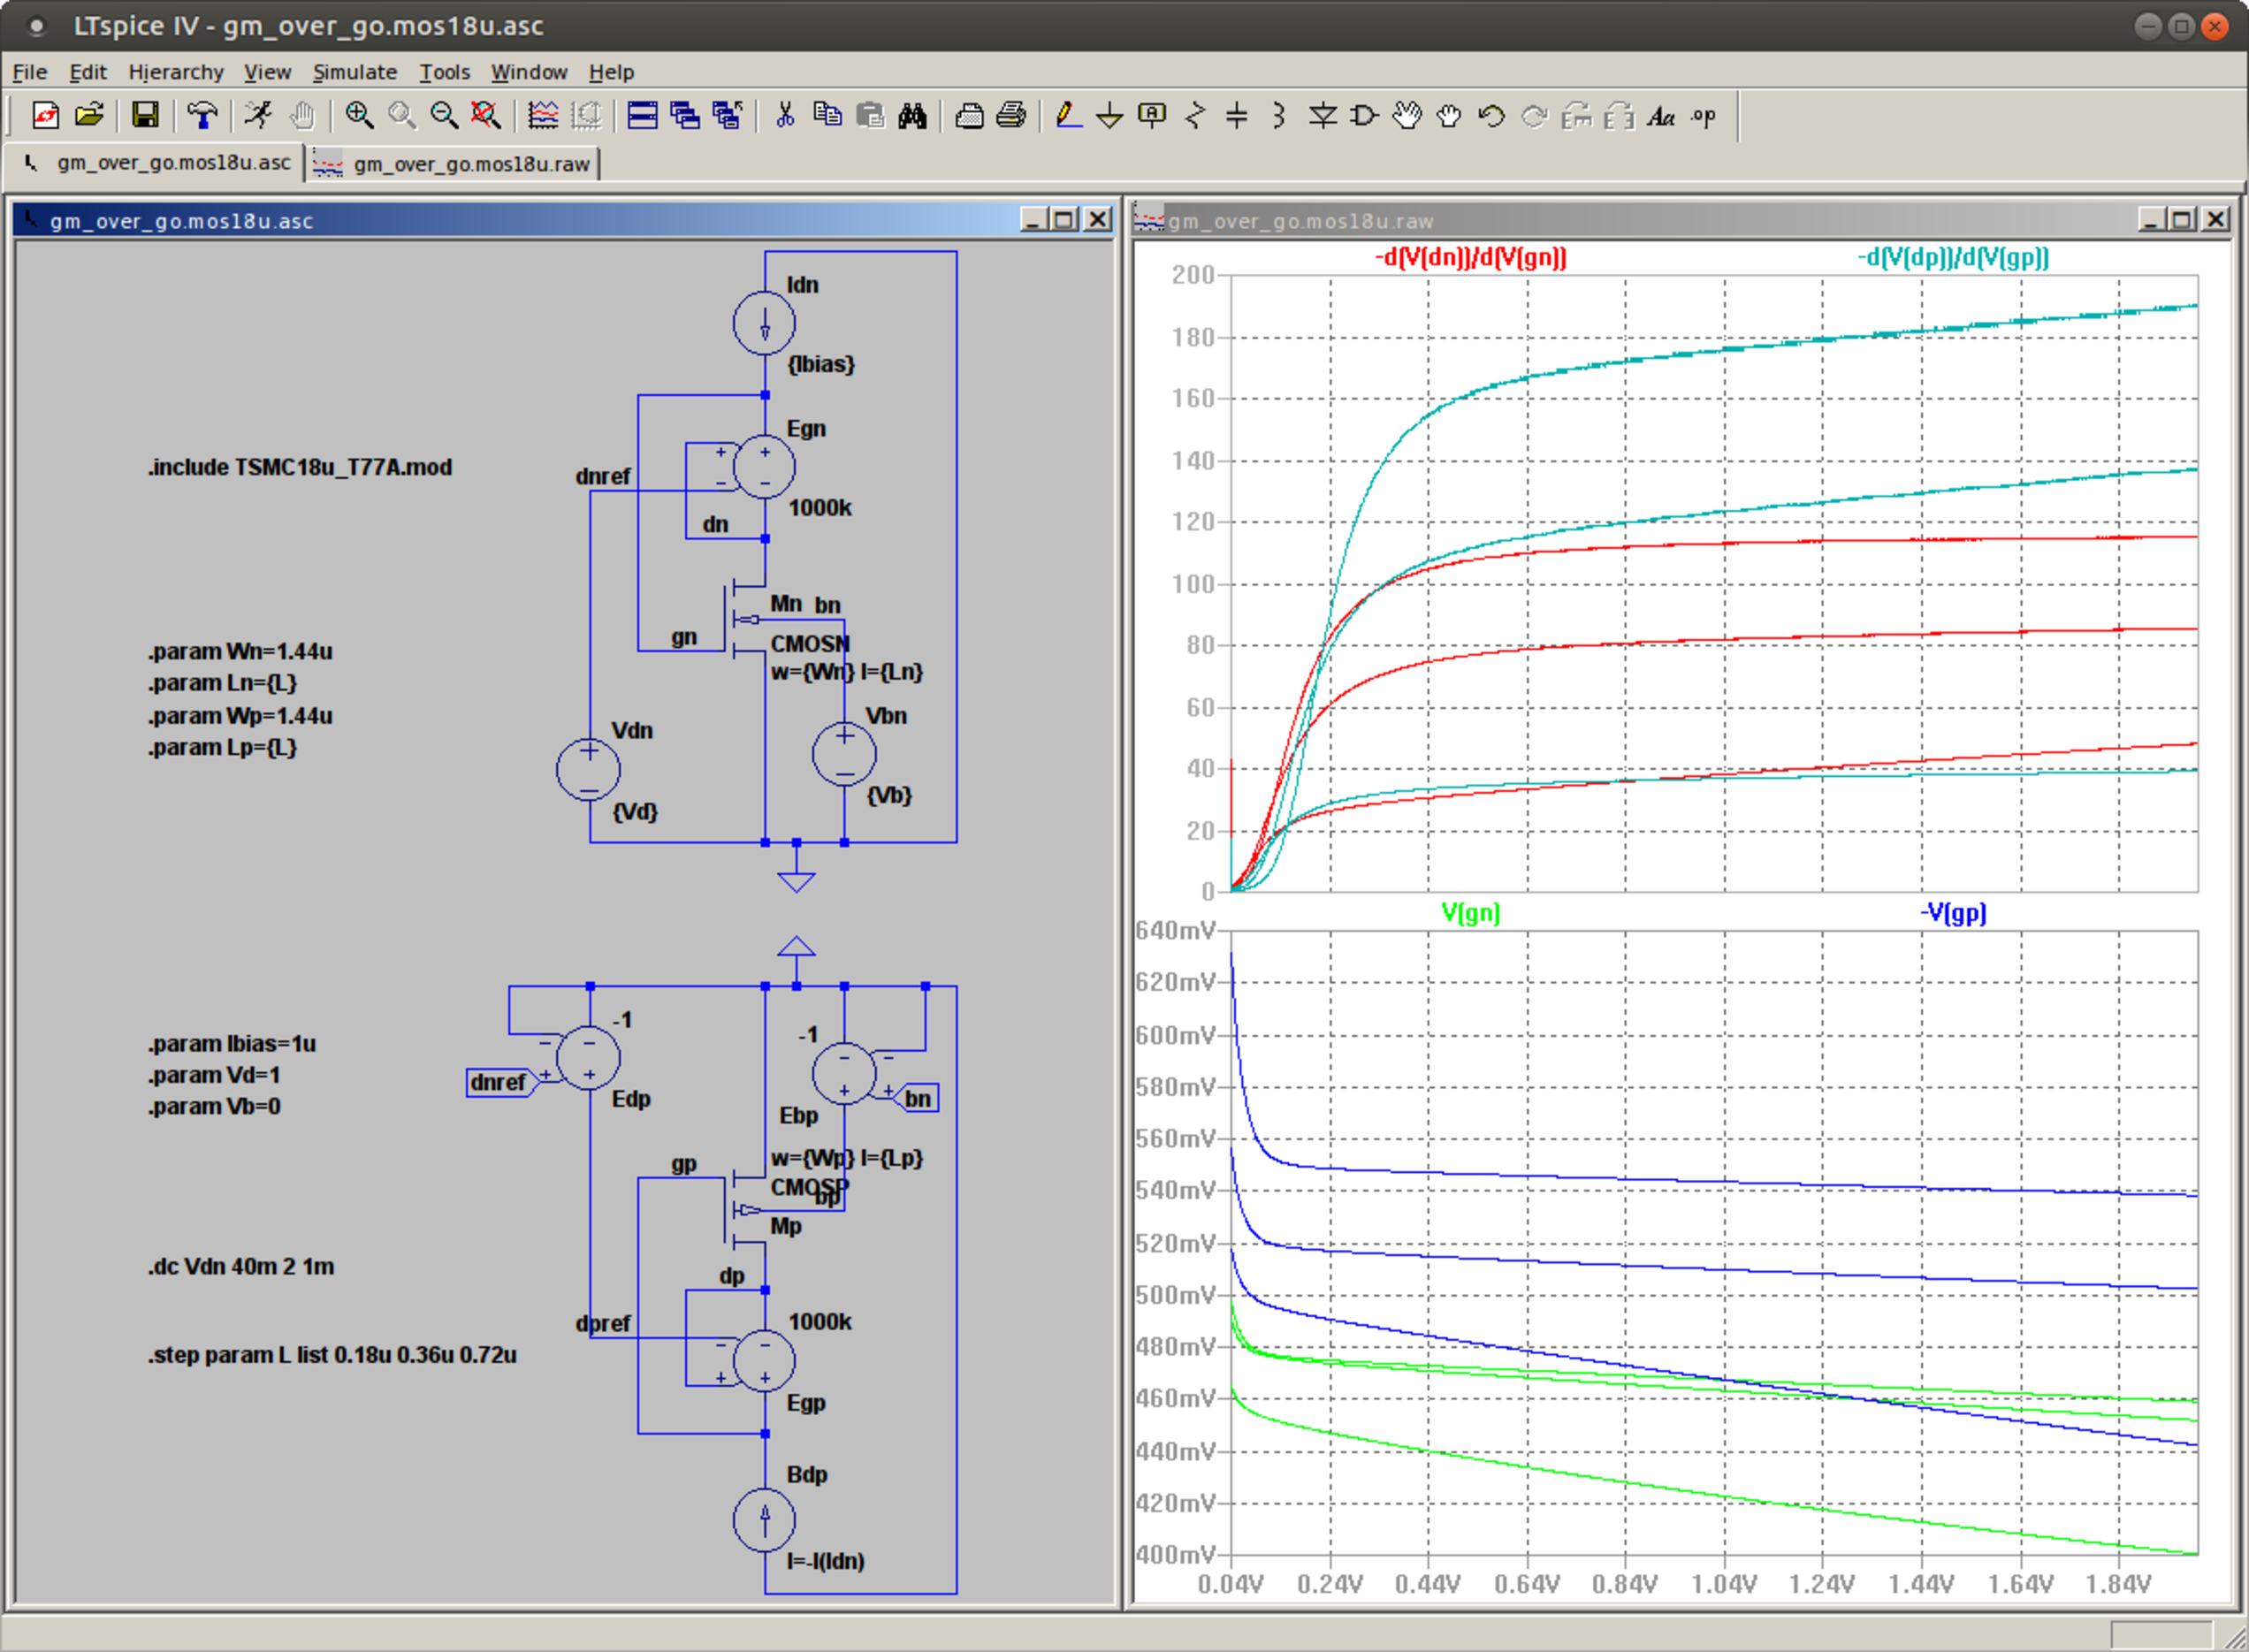
\includegraphics[width=1.0\columnwidth]{figures/gm_over_go_mos18u.pdf}
\caption{Voltage gain characterization for 180\,nm process}
\label{fig:gm_go_mos18}
\end{figure}
%

For the dc voltage gain of a transistor stage, 
the transconductance to output conductance ratio $g_m/g_o$ is the key figure of merit.
$g_o$ depends on transistor length and drain-to-source voltage $V_{d{s}}$ 
in a way too complicated for hand calculations. 

A linear sweep of~$V_d$ at constant~$I_d$ allows to optimize transistor length 
and minimum required~$V_{d{s}}$ to achieve the best possible voltage gain
within design constraints for the process. 
$g_m$ and $g_o$ are obtained by taking the derivatives of $V_g$ and $V_d$ with respect to the dc sweep variable $V_d$, and calculating the ratio
\begin{equation}
\frac{g_m}{g_o} = -\frac{\mathrm{d}\le(V_d\ri)}{\mathrm{d}\le(V_g\ri)}
\end{equation}
due to the implicit relation for constant $I_d$
\begin{equation}
g_o\,\mathrm{d}\le(V_d\ri) + g_m\,\mathrm{d}\le(V_g\ri) = 0\,.
\end{equation}

Figures \ref{fig:gm_go_mos25} and~\ref{fig:gm_go_mos18}
show LT\,Spice\,IV linear $V_d$ dc sweeps at different transistor lengths for two different processes 
(TSMC~250\,nm and TSMC~180\,nm).

Longer transistors have a higher $g_m/g_o$, PMOS can achieve higher $g_m/g_o$ than NMOS,
and the process with larger minimum feature size has higher maximal $g_m/g_o$.

\section{Conclusion}
%%
I present a single transistor simulation circuit, 
first published in the LT\,Spice Yahoo group in~2008~\cite{Yahoo2008},
with feedback control of the gate voltage~$V_g$
together with a method to dc sweep both 
$I_d$ for constant~$V_d$ and $V_d$ for constant $I_d$
and a method to compute 
\begin{equation}
g_m = \frac{\mathrm{d}\le(I_d\ri)}{\mathrm{d}\le(V_g\ri)} \quad\mathrm{and}\quad
\frac{g_m}{I_d} = \frac{\frac{\mathrm{d}\le(I_d\ri)}{\mathrm{d}\le(V_g\ri)}}{I_d}
\end{equation}
from the $I_d$ sweep, and
\begin{equation}
\frac{g_m}{g_o} = -\frac{\mathrm{d}\le(V_d\ri)}{\mathrm{d}\le(V_g\ri)}
\end{equation}
from the $V_d$ sweep. 

This simulation circuit is suitable
\begin{itemize}
\item to get a quick overview of the properties of an unfamiliar IC process
\item to set the dimension and bias points of transistors 
\item to design circuits using the $g_m/I_d$ methodology.~\cite{Silveira1996}
\end{itemize}

Coincidentally, the same feedback circuit, but without the parameter extraction methods, 
has been published in~\cite{Bruun2017}.

\begin{thebibliography}{1}
\bibitem{Silveira1996}
F.~Silveira, D.~Flandre, P.\,G.\,A.~Jespers,
\textsl{``A $g_m/I_D$ based methodology for the design of CMOS analog circuits and its application to the synthesis of a silicon-on-insulator micropower OTA''},
IEEE Journal of Solid-State Circuits vol.~31 no.~9, Sep.~1996, pp.~1314--1319,
doi:10.1109/4.535416

\bibitem{Yahoo2008}
C.~Maier, \textsl{``Badenke und Klee''}, File directory, LTspice Yahoo group, April~2008,\\
URL: \url{https://groups.yahoo.com/neo/groups/LTspice/files/Badenke\%20und\%20Klee/}

\bibitem{Bruun2017}
E.~Bruun, \textsl{``CMOS Integrated Circuit Simulation with LTspice''}, Figure~3.30, 
bookboon.com, $2^{nd}$~ed.~2017, $1^{st}$~ed.~2015,\\
URL: \url{https://bookboon.com/en/cmos-integrated-circuit-simulation-with-ltspice-ebook}
\end{thebibliography}

\end{document}


http://web02.gonzaga.edu/faculty/talarico/EE406/documents/gmid.pdf

http://www.mos-ak.org/sanfrancisco/papers/08_Jespers_MOS-AK_SF08.pdf
